\renewcommand{\thefigure}{A\arabic{figure}}
\renewcommand{\thetable}{A\arabic{table}}
\setcounter{figure}{0}
\section{Apêndice}
\subsection{Regeneração da portadora com PLL}
\label{subsec:PLL}

%\iffalse
\begin{figure}[H]
    \centering
    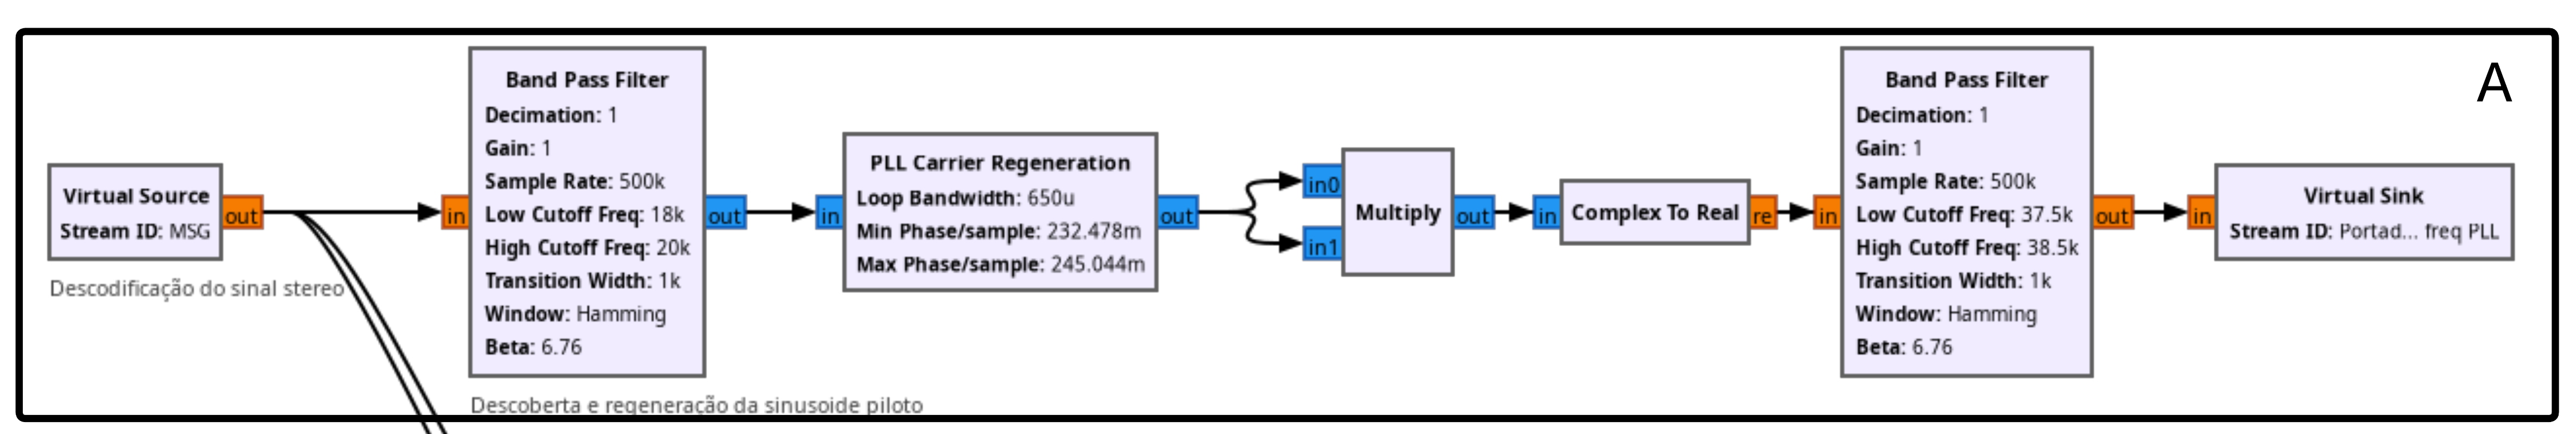
\includegraphics[width = 0.9\linewidth]{img/appendix/PLL_galore.png}
    \caption{Esquema de regeneração da portadora e duplicação de frequência com o PLL.}
    \label{fig:appendix0}
\end{figure}
%\fi

O processo de regeneração da portadora, analisado no \hyperref[subsec:mod3]{módulo 3}, pode ser efetuado com o auxilio de um bloco \textit{"PLL Carrier Regeneration"}. A seguinte \hyperref[fig:appendix1]{Fig. A2} ilustra o funcionamento genérico de um PLL. 
\vspace{0.5em}
\iffalse
\begin{figure}[H]
    \centering
    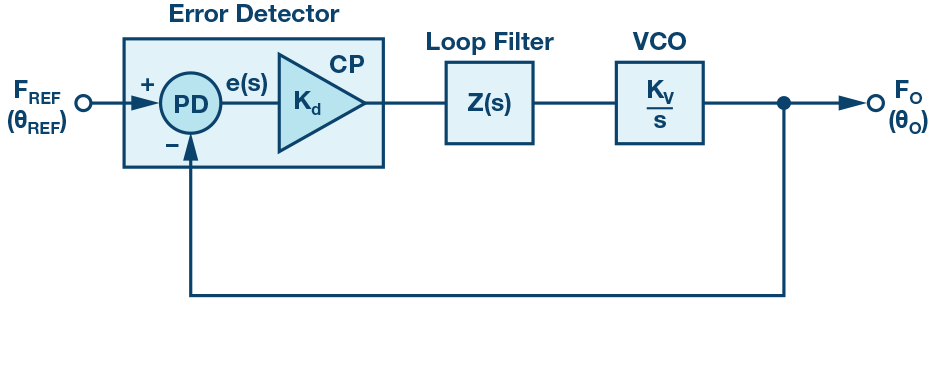
\includegraphics[width = 0.55\linewidth]{img/appendix/PLL.png}
    \caption{Configuração genérica do PLL.}
    \label{fig:appendix1}
\end{figure}
\fi

\begin{tabular}{C{8cm}  L{6.5 cm}}
        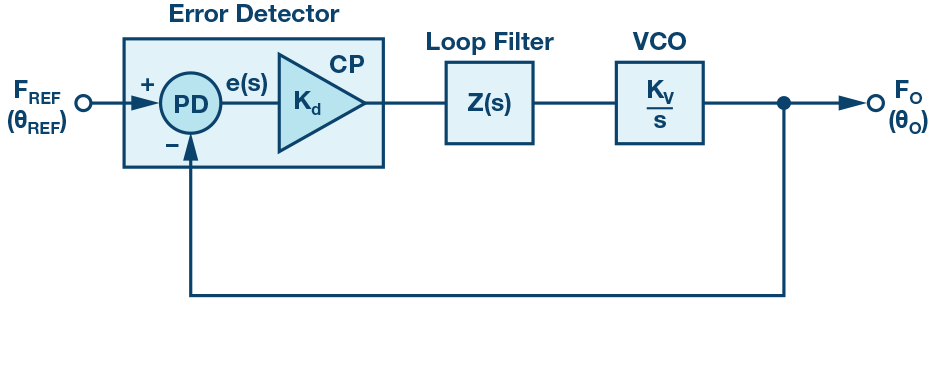
\includegraphics[width=\linewidth]{img/appendix/PLL.png}\captionof{figure}{Configuração genérica do PLL\cite{person}.} & 
        Dado que ultrapassa o âmbito da UC, procedemos apenas a uma análise empírica do bloco supramencionado que: \textit{"(...) locks onto a [possibly noisy] reference carrier on the input and outputs a clean version which is phase and frequency aligned to it."}\cite{pll_ref_out-gnuradio}
    \end{tabular}
    
\vspace{0.5em}
\noindent\fcolorbox{black}{white}{%
    \minipage[t]{\dimexpr\linewidth-2\fboxsep-2\fboxrule\relax}
        \textbf{Observação 1} $\rightarrow$ Após uma análise espectral da portadora regenerada, verificou-se, de facto, uma versão mais limpa do sinal de entrada, que nos é favorável dado que pretendemos eliminar ao máximo o ruído nos sinais auxiliares na descodificação da mensagem. No entanto, o fator $K$ da subportadora piloto perde-se neste processo e a portadora que sai do PLL dispõe de uma amplitude unitária.
    \endminipage}
\newline\break
\noindent\fcolorbox{black}{white}{%
    \minipage[t]{\dimexpr\linewidth-2\fboxsep-2\fboxrule\relax}
        \textbf{Observação 2} $\rightarrow$ Visto que uma emissora de sinal FM em Lisboa, tipicamente não transmite conteúdo stereo (i.e., o sinal tem tipicamente formato stereo, mas o conteúdo da esquerda é equivalente ao da direita, $L=R$), o facto da amplitude da portadora regenerada ser unitário acaba por comprometer a qualidade sonora audível, dado que eleva o ruído de fundo proveniente da fase de deteção coerente da componente $L-R$ (que deveria ser nula teoricamente, mas apresenta-se como uma camada de ruído). 
    \endminipage}
\newline\break
Devido a estas duas observações, foi decidido não apresentar esta solução como principal, visto que compromete a qualidade sonora audível. No entanto, é importante porque salienta a existência de outros métodos de recuperação da portadora, e passando à citação:

\textit{"(...) PLL chips now relatively cheap, (...) PLL applications enables high quality audio to be demodulated from an FM signal."}\cite{notes}